\section{A Shape-Diverse FSM Language}
\label{sec:eval}

To illustrate \prism, we built a shape-diverse FSM language conjointly in Rascal, EMF, and Java.
\Cref{fig:3fsms} depicts the implementation of the abstract syntax of this FSM language in the three LVs.\footnote{The implementation of \prism and the FSM example are available on a companion webpage:~\url{https://github.com/fcoulon/prism/}}
The corresponding incarnations are given in \Cref{fig:motivating-fsm}.

\begin{figure}[bt]
	\centering
	\begin{subfigure}[b]{.3\columnwidth}
		\begin{lstlisting}[label=lst:fsm-adt, language=Rascal, numbers=none, xleftmargin=0pt, tabsize=1]
data Machine(Id uid) =
	Machine(str name,
		list[State] states,
		Ref[State] initial);

data State(Id uid) =
	State(str name,
		list[Trans] trans);

data Trans(Id uid) =
	Trans(str event,
		Ref[State] target);
		\end{lstlisting}
		\caption{Rascal ADT}
	\end{subfigure}
	\vrule
	\enskip
	\begin{subfigure}[b]{.26\columnwidth}
		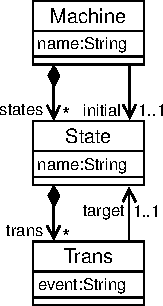
\includegraphics[width=\textwidth]{figures/fsm-mm}
		\caption{Ecore MM}
	\end{subfigure}
	\enskip
	\vrule
	\enskip
	\begin{subfigure}[b]{.35\columnwidth}
		\begin{lstlisting}[label=lst:fsm-api, language=Java, numbers=none, xleftmargin=0pt, tabsize=1]
class Fsm {
	Fsm(String name);
	State init(String name);
	State state(String name);
	Fsm end();
}
class State {
	State state(String name);
	Trans tgt(String name);
	Fsm end();
}
class Trans {
	Trans tgt(String name);
	State on(String event);
	Fsm end();
}
		\end{lstlisting}
		\caption{Java API}
	\end{subfigure}
	\caption{Three shapes of an FSM language; the corresponding incarnations are those depicted in \Cref{fig:motivating-fsm}.}
	\label{fig:3fsms}
\end{figure}

We use Rascal to define a textual editor and a simple transformation that inserts a new state in a machine.
We use EMF to define two graphical editors:~a classical tree editor and a domain-specific representation with Sirius.\footnote{\url{https://www.eclipse.org/sirius/}}
We build the Java API following a simple systematic convention, so that we can easily pinpoint which parts of the Java AST have changed (to compute a patch) or need to be updated (to apply a patch).

\prism is used to bridge these different shapes.
Whenever an incarnation of the FSM model is updated, the LV in which the change happens produces a patch (\cf\Cref{lst:delta-adt}) that is shipped to the other LVs.
Every LV interprets the patch in its own way to keep its incarnation updated, accounting for the extra information it has to manage (\eg~layouts within the textual and graphical editors).
A simple matrix, internal to \prism, keeps track of which model each incarnation is projecting to route the patch to the right incarnation.

%Rascal is providing a textual editor, Ecore provides a graphical editor and we used the Java editor for the fluent API.
%In our manipulation we were able to edit an incarnation of a model in one editor and see the change applied in others editors.
%By using an editor, we were able to benefit of the result of the tooling in others incarnations, i.e., using the content assist of Java is also updating other editors.
%We also observe some de-synchronization happening due to the partially unaligned FSM implementation in Java.

While the Rascal and EMF shapes synchronize seamlessly, we noticed a number of problems with the Java API.
As the Java API inherits the (domain-agnostic) tooling of Java itself, it lacks the domain knowledge necessary to always generate correct patches.
Due to the lack of domain-specific static semantics, a well-formed Java program may indeed produce an ill-formed FSM that cannot be interpreted by the other shapes.
Besides, our prototype implementation does not account for complex string manipulation when invoking the API or use of variables.
However, we believe that these are purely engineering concerns and that enough effort spent on the Java API shape would provide a flawless experience.

%The Java fluent API shape tends to break more easily the synchronization of their incarnations of models than the other shapes.
%Indeed this shape of FSM language is an embedded language and has to rely on the host language for both the tooling and the expressiveness.
%In the case of Java as host language, the validation service provided by the editor has no knowledge about the FSM language.
%It makes harder for the user to detect mistakes such as typo. The FSM model can be in unnoticed dirty state and this can lead to the production of dirty Patches.
%In the opposite the incarnation of the model can receive inapplicable Patches in this technological space.

%Another example in the Java TS of problem encountered is the constraints from the host language.
%We choose to represent a State by the method state() or by the method initial().
%As the initial State is unique, we enforce its declaration as the first method invocation in the FSM.
%This solution solve the uniqueness but enforce the first state to be initial.
%Thus with this representation of FSM, receiving a Patch telling to reference the second state of an FSM as the initial state is not possible due to the expressiveness of the API and this result in the desynchronization of the incarnation of the model.
%
%The inconsistency of the incarnations of a model happen when one of them produce a dirty Patch or when one of them can't apply a Patch.
